\documentclass[a4paper,twoside]{book}
\usepackage{rutitlepage}
\usepackage{url}
\usepackage{geometry}
\usepackage[english]{babel}
\usepackage{lipsum,etoolbox}
\usepackage[nodayofweek]{datetime}
\usepackage[toc,acronym,shortcuts]{glossaries}
\usepackage{listings}
\usepackage{float} % Pictures
\usepackage[backend=biber,style=numeric]{biblatex}
%\usepackage{courier} % Clean syntax highlighting
\usepackage{subcaption} %subfigure
\usepackage[export]{adjustbox} % subfigure
\usepackage{graphicx} %subfigure
\usepackage{lmodern}


\addbibresource{thesis/thesis.bib}

\usepackage{listings}
\usepackage{stmaryrd}

% color definitions
% the following colors are appealing for background of code segments
%CornflowerBlue    heldere blauwe kleur
%CadetBlue         sobere blauwe kleur
%Periwinkle        blauw die neigt naar paars, nogal donker
%Thistle           wat valere kleur, minder nadrukkelijk aanwezig
%YellowOrange      erg nadrukkelijke kleur
\newcommand{\ExampleCodeBackgroundColor}{\color{White}}
\newcommand{\ExampleCodeFrameColor}{\color{black}}
\newcommand{\CleanDocFrameColor}{\color{black}}


\lstdefinelanguage{Clean}{%
	alsoletter={ABCDEFGHIJKLMNOPQRSTUVWXYZabcdefghijklmnopqrstuvwxyz_`1234567890},
	alsoletter={~!@\#$\%^\&*-+=?<>:|\\.\\{\\}},
	morekeywords={generic,implementation,definition,dynamic,module,import,from,where,in,of,case,let,infix,infixr,infixl,class,instance,with,if,derive,code},
	sensitive=true,
	escapeinside={[+}{+]},
	morecomment=[l]{//},
	morecomment=[n]{/*}{*/},
	morestring=[b]",
	morestring=[s]{['}{']},
	basewidth=0.43em,
	columns=[c]fixed,
	texcl=true,
	literate=%
		% Basic Clean constructs
		{\\}{{$\lambda\:$}}1
		%{::}{{$:\!\!\!:$}}1
		%{:.}{{$:\!.$}}1
		{...}{{.\!.\!.}}2
		%{++}{{$+\!+$}}2
		%{+++}{{$+\!\!\!+\!\!\!+$}}2
		%{==.}{{==\!.}}2
		%{=.}{{=\!.}}1
		%{>=}{{$\geq\:$}}1
		%{<=}{{$\leq\:$}}1
		%{||-}{{$\mid\mid\!$-}}2
		%{-||}{{-$\!\mid\mid$}}2
		%{-||-}{{-$\!\mid\mid\!$-}}2
		%{-&&-}{{-$\!\&\!\&\!$-}}4
		{not}{{$\neg$}}1
		{->}{{$\shortrightarrow$}}1
		{<<@}{{$\ll\!\!@$}}2
		%{>>=}{{$\gg\!\!=$}}2
		%{>>*}{{$\gg\!\!\!\!^*$}}2
		%{>>|}{{$\gg\!\mid$}}2
		{A.}{{$\forall\;\,$}}1
		%{E.}{{$\exists\;\,$}}1
}


\lstdefinestyle{cleanStyleInline} {
    breakatwhitespace,
    breaklines
}

\newcommand{\CleanInline}[1]{\lstinline[language=Clean,style=cleanStyleInline];#1;}
\newcommand{\Cl}[1]{\CleanInline{#1}}
\newcommand{\CI}[1]{\lstinline[language=Clean,basicstyle=\ttfamily\fontseries{l}\normalsize]|#1|}

\lstdefinestyle{numbers}{numbers=right, stepnumber=1, numberstyle=\tiny, numbersep=-5pt}

% environments for documentary code segments
\lstnewenvironment{CleanDoc}{\lstset{language=Clean}}{}
\lstnewenvironment{CleanDocN}{\lstset{language=Clean,style=numbers}}{}
\lstnewenvironment{CleanDocB}{\lstset{language=Clean,frame=single,rulecolor=\CleanDocFrameColor}}{}
\lstnewenvironment{CleanDocNB}{\lstset{language=Clean,style=numbers,frame=single,rulecolor=\CleanDocFrameColor}}{}

% environments for example code segments
\lstnewenvironment{CleanEx}{\lstset{language=Clean,frame=single}}{}
\lstnewenvironment{CleanExN}{\lstset{language=Clean,style=numbers,frame=single,rulecolor=\ExampleCodeFrameColor,backgroundcolor=\ExampleCodeBackgroundColor}}{}

\lstset{
    language=Clean,
    showstringspaces=false,
    basicstyle=\ttfamily,
    frame=leftline}

\makeglossaries
\newacronym{adt}{ADT}{Algebraic Data Type}

\newacronym{dsl}{DSL}{Domain Specific Language}

\newacronym{edsl}{E\acs{dsl}}{Embedded \acl{dsl}}

\newacronym{gadt}{GADT}{Generalized Algebraic Data Type}

\newacronym{gpl}{GPL}{General Purpose Language}

\newacronym{html}{HTML}{Hypertext Markup Language}

\newacronym{iot}{IoT}{Internet of Things}

\newacronym{sds}{SDS}{Shared Data Source}

\newacronym{top}{TOP}{Task Oriented Programming}

\newacronym{vhdl}{VHDL}{\acs{vhsic} Hardware Description Language}

\newacronym{vhsic}{VHSIC}{Very High Speed Integrated Circuit}

\newacronym{led}{LED}{Light-Emitting Diode}

\newacronym{mcu}{MCU}{Microcontroller Unit}

\newacronym{midi}{MIDI}{Musical Instrument Digital Interface}

\newacronym{eeprom}{EEPROM}{Electrically Erasable Programmable Read-Only Memory}

\newacronym{ghc}{GHC}{Glasgow Haskell Compiler}

\newacronym{uav}{UAV}{Unmanned Air Vehicles}

\newacronym{frp}{FRP}{Functional Reactive Programming}

\newacronym{ota}{OTA}{Over-the-Air}

\newacronym{ide}{IDE}{Integrated Development Environment}

\urlstyle{tt}

\newcommand{\projecttitle}{Developing Real Life, Task Oriented Applications for the Internet of Things}
\newcommand{\rinus}{prof.~dr.~dr.h.c.~ir.~M.J.~Plasmeier }
\newcommand{\pieter}{dr.~P.W.M. Koopman}
\newcommand{\mart}{M. Lubbers MSc.}

\date{\today}
\author{Matheus Amazonas Cabral de Andrade}

\begin{document}
\maketitleru[
    layout=seventeen,
    title=Master's Thesis,
    subtitle=\projecttitle,
    others={{Supervisor:}{\rinus},{Daily Supervisor:}{\mart},{Second Reader:}{\pieter}}]
    
\clearpage

\chapter*{\centering Abstract}
    \addcontentsline{toc}{chapter}{Abstract}
    
   Lorem ipsum dolor sit amet, consectetur adipiscing elit. Nulla urna libero, hendrerit eget tempor a, pulvinar vitae metus. Interdum et malesuada fames ac ante ipsum primis in faucibus. Aenean id tellus consectetur, mattis ipsum eget, vehicula tortor. Sed nec sodales magna, nec volutpat ex. Donec faucibus malesuada nunc, vel ullamcorper dui cursus in. Fusce ante sem, posuere non ultricies eget, gravida varius nibh. Phasellus rutrum sit amet sapien quis ultrices. Pellentesque sollicitudin eros eu rhoncus tempor.
    
\chapter*{\centering Acknowledgements}
    \addcontentsline{toc}{chapter}{Acknowledgements}
    Lorem ipsum dolor sit amet, consectetur adipiscing elit. Nulla urna libero, hendrerit eget tempor a, pulvinar vitae metus. Interdum et malesuada fames ac ante ipsum primis in faucibus. Aenean id tellus consectetur, mattis ipsum eget, vehicula tortor. Sed nec sodales magna, nec volutpat ex. Donec faucibus malesuada nunc, vel ullamcorper dui cursus in. Fusce ante sem, posuere non ultricies eget, gravida varius nibh. Phasellus rutrum sit amet sapien quis ultrices. Pellentesque sollicitudin eros eu rhoncus tempor.

\tableofcontents
\clearpage

\chapter{Introduction}
    \section{Introduction}
% Structure: 
%   IoT
%   TOP and iTasks
%   mTask
The \ac{iot} consists of a network of ``things'' (devices, computers, people, systems, etc.) that interact with each other via the Internet. These components can exchange data, monitor and manage each other. \ac{iot} is a global, growing phenomenon. According to Gartner, there were 3.96 billion connected ``things'' in 2016 and by 2020, 12.863 billion devices are expected to be connected to the Internet~\cite{iot_numbers}. \ac{iot} has been used in a myriad of applications including home automation, fitness tracking, health care, warehouse monitoring, agriculture and industry manufacturing. \ac{iot} devices can be dedicated servers, personal computers, tablets, smartphones, smartwatches or compact devices operated by microcontrollers. Microcontrollers are small, cheap computers with limited resources and low power consumption commonly used to interface with the real world. They often gather data from sensors (movement, light, temperature, etc.), act on actuators (motors, \acsp{led}, switches, etc.) and communicate with other devices.

\ac{top} is a new programming paradigm used to develop online, collaborative applications. Its central concept, a \textit{task}, can be used to model different types of work performed both by users and systems. \ac{top} provides a high level of abstraction, liberating the programmer from the burden of technical details, such as user interfaces. The iTasks~\cite{top} system implements \ac{top} in the functional programming language Clean~\cite{clean} as an \ac{edsl}. It automatically generates as many assets as possible, turning it into a great tool for rapid prototyping. Given an iTasks program, the system automatically generates a web application that can be accessed via a web browser. Users can access this application to inspect and work on tasks. The system has been proved useful in many fields, including incident response operations and navy vessels automation~\cite{incidone,navy}.

Although iTasks applications often require user interaction, some tasks could be automated. Examples are tasks that interact with the external world: reading room temperature, blinking an \acs{led}, detecting movement, unlocking a door,  etc. The iTasks environment could benefit from such automation. Microcontrollers pose as great candidates to interface with the external world. They are affordable, energy efficient and are seamlessly combined with sensors and actuators. Unfortunately, --- due to hardware limitations --- microcontrollers are not suitable to run iTasks tasks. To bridge this gap, the mTask \ac{dsl} was created to enable the execution of simple tasks on microcontrollers, bringing such devices to the iTasks world.


\section{Research Question}
Even though mTask was created to allow iTasks tasks to run on \acs{iot} devices, it has not been proved capable of running real-life applications yet. The examples built during its development were simple demonstrations and were far from real-life \acs{iot} applications. Given that, I propose the following research question:

\begin{center}
\emph{Is it possible to develop real-life, \acs{iot} applications using mTask? If so, how can the development process be improved? If not, what are the challenges to solve to make it possible?}
\end{center}
I plan to tackle the research question by example. Namely, trying to develop a real life \acs{iot} application using mTask. The attempt to develop such an application should display mTask's capability to create real life applications while displaying new opportunities to improve the development process.

The application I chose to develop tackles a popular problem in \acrshort{iot}: home automation. This application would be responsible for automating simple home management tasks such as turning the central heating system off when the room is warm, or opening up the curtains at a set time. The proposed application requires several \acrshort{iot} devices equipped with sensors (temperature, light, humidity, etc.) and actuators (\acsp{led}, motors, relays, etc.) spread across rooms. 


\section{Report Structure}

This report is structured as follows. \cref{chap:intro} contains the introduction, research question and report structure. \cref{chap:edsl} quickly introduces \acp{dsl} and presents different strategies to build \acp{edsl}. \cref{chap:top} introduces the concept of \ac{top} and the iTasks system. \cref{chap:mtask} presents the mTask \ac{edsl}, which was the research focus. \cref{chap:application} describes the real-life application developed during research. \cref{chap:dev} details the development process. \cref{chap:conclusion} concludes presenting insight about the development process, answering the research question and proposing future research. \cref{chap:related} lists related work.

The source code for the real-life application developed during research can be accessed at \url{https://github.com/matheusamazonas/autohouse}.

The source code of the modified version of mTask used during research can be accessed at \url{https://gitlab.science.ru.nl/mlubbers/mTask/tree/peripherals}.

The source code of this report can be accessed at \url{https://github.com/matheusamazonas/masterthesis}.

%The source code of the library to interface with the DHT22 temperature and humidity sensor can be accessed at \url{https://github.com/matheusamazonas/DHTino}.

%The source code of the library to interface with the HC-SR04 ultrasonic sensor can be accessed at \url{https://github.com/matheusamazonas/Ultrino}.

\chapter{Embedded Domain Specific Languages}
    A \ac{gpl} is a computer language intended to be used in a wide range of domains. An example is the C++ programming language, which can be used in domains that vary from video games to web servers and systems programming. In contrast, a \ac{dsl} is a computer language that was designed to be used in a particular domain. Game Maker Language, \acs{html}, LaTeX and \acs{vhdl} are examples of \acp{dsl}. These languages, when compared to \acp{gpl}, offer a higher level of abstraction from their target domain.

A \ac{dsl} can be implemented using two different strategies: standalone and embedded. Each strategy has its advantages and disadvantages. In the former strategy, the language is build from the ground up, which consists of developing either a compiler or an interpreter. This strategy provides the language designer with a lot design freedom, but requires a cumbersome amount of work. In the latter strategy, the proposed \ac{dsl} is embedded in another language. This strategy frees its designer of building a new compiler, but limits the \ac{dsl} to the features of its host language.

The semantics of a \ac{edsl} are given by its views (also called backends). Common views are evaluation, pretty printing, compilation, optimization and verification. There are two main techniques for building an \ac{edsl}: deep and shallow embedding.

\section{Deep Embedding}

Building a deeply \ac{edsl} consists of representing language constructs as \acp{adt} in the host language. Views are functions that take the \ac{adt} as input and return another \ac{adt} that represents its semantics. An example of a simple deeply \ac{edsl} and its views (pretty printing and evaluation) can be seen on Listing \ref{deep1}.


\begin{lstlisting}[caption=A simple deeply \ac{edsl} and its views,captionpos=b,label=deep1]
:: MyDSL = I Int
    | B Bool
    | Add MyDSL MyDSL
    | Sub MyDSL MyDSL
    | And MyDSL MyDSL
    | Or MyDSL MyDSL
    | Var String
    
prettyPrint :: MyDSL -> [String]
eval :: MyDSL -> Int
\end{lstlisting}

The biggest advantage of deep embedding is that adding a view to the \ac{dsl} is easy: simply create a function that transforms the \ac{adt}. One disadvantage is that extending the \ac{dsl} might require a lot of work, since new code has to be created for every new construct in all the views. Another disadvantage is its lack of static type safety. As seen on Listing \ref{deep1}, \texttt{MyDSL} allows operations on mixed data types, as addition on booleans and disjunction on integers. In addition, variables are checked at runtime instead of compile time.

\acp{gadt} can be used to accomplish static type safety in deeply \acp{edsl}, but they not enable compile time variable checks. 

\section{Shallow Embedding}
Building a shallowly \ac{edsl} consists of representing the language constructs directly as its semantics. An example of a simple shallowly \ac{edsl} can be seen on Listing \ref{shallow1}.

\begin{lstlisting}[caption=A simple shallowly \ac{edsl},captionpos=b,label=shallow1]
:: Sem a = Sem (a, [String])

add :: (Sem a)    (Sem a)    -> Sem a    | + a
and :: (Sem Bool) (Sem Bool) -> Sem Bool
eq ::  (Sem a)    (Sem a)    -> Sem Bool | == a
var :: String -> Sem Int
\end{lstlisting}

One advantage of shallow over deep embedding is that adding a new language construct is easy, given that each construct is just a function. Another advantage is that overloading can be achieved with the use of class constraints. In addition, static type checking was obtained without \acp{gadt}. 

The biggest disadvantages of shallow embedding are based on the fact that all views will always be computed regardless of its need. First, there is no separation of concerns. Second, there is computational waste when not all views are necessary. Finally, adding a new view in the semantics becomes increasingly burdensome. Another disadvantage of shallow embedding is that variables still remain unchecked during compilation. Finally, since the language constructs are functions, they can not be inspected as in deeply \acp{edsl}.

\subsection{Shallow Embedding with Type Classes}

Type classes can be used to avoid computing all the views of a shallowly \ac{edsl}. A type class containing the language constructs is created and each of the \ac{dsl} views should provide an instance of the class. An example of a simple shallowly \ac{edsl} with classes can be seen on Listing \ref{shallow2}.

\begin{lstlisting}[caption=A simple shallowly \ac{edsl} with classes,captionpos=b,label=shallow2]
:: Print a = P [String]
:: Eval a = E a

class myDSL v where
    lit :: t -> v t | toString t
    add :: (v t)    (v t)    -> v t    | + t
    and :: (v Bool) (v Bool) -> v Bool
    eq  :: (v t)    (v t)    -> v Bool | == t
    
instance myDSL Print where
    lit x = P [toString x]
    add (P x) (P y) = P (x ++ [" + ":y])
    and (P x) (P y) = P (x ++ [" && ":y])
    eq  (P x) (P y) = P (x ++ [" == ":y])
    
instance myDSL Eval where
    lit x = E x
    add (E x) (E y) = E (x + y)
    and (E x) (E y) = E (x && y)
    eq  (E x) (E y) = E (x == y)
\end{lstlisting}

Class-based shallow embedding solves most of the problems previously faced with deep and shallow embedding. The language is statically typed, the views are separated, adding a view is simple, extending the language with a new construct is easy and operators can be overloaded. 

Two problems remain. First, language constructs still can not be inspected. This is an inherent property of shallowly \acp{edsl} and unfortunately can not be eliminated. 

Second, variables are still not checked at compile time. In order to solve this problem, we can leverage the fact that function arguments are well typed in the host language. A variable declaration is defined as a function where its argument represent the variable and the function body represents the remaining of the program. As a result, any usage of the variable in the function body is well typed. An example of a class-based shallowly \ac{edsl} with compile time variable checks can be seen on Listing \ref{shallow3}.

\begin{lstlisting}[caption=A simple shallowly \ac{edsl} with compile time variable checks,captionpos=b,label=shallow3]
:: Eval a = E a
:: In a b = In infixl 0 a b

class expr v where
    lit :: t -> v t
    (+.) infixl 6 :: (v t) (v t)  -> v t
    
class var v where
    var :: ((v t) -> In t (v a))   -> v a
    ( =. ) infixr 3 :: (v t) (v t) -> v t

instance expr Eval where ...
instance var Eval where ...

test1 :: Eval Int	
test1 = var \k = 4 In
	k  =.  k + lit 7

test2 :: Eval Int	
test2 = var \k = 4 In
	k  =.  lit True     // Compilation error
\end{lstlisting}

As seen in the example above, the variable \texttt{k} can be used after its declaration in a well typed manner. Function \texttt{test1} compiles successfully, as expected. Function \texttt{test2}, in the other hand, does not compile due to a type error. Therefore, compile time check of variables was achieved.



\chapter{Task Oriented Programming}
    \acf{top} is a new programming paradigm used to develop online collaborative applications. In a \acs{top} application, users - both people and other systems - work together to accomplish a common goal. Its central concept is called a Task, an abstraction that can be used for many different types of work. This abstraction, along with other TOP concepts, allows the user to focus on design decisions instead of technical details. TOP programs are declarative: they focus on \textit{what} work the user performs, rather than on \textit{how} to perform it.

\section{iTasks}\label{itasks}
iTasks is an \acs{edsl} that implements the \acs{top} paradigm. Its host language is the pure and lazy functional programming language \textit{Clean}. iTasks uses generic programming to automatically generate code for user-specified data types whilst also allowing for specialization. Given an iTask program, the system generates code for both the server and the client.

An iTask Task is a function that consumes a state and returns a \texttt{TaskValue} of type \texttt{a}, where \texttt{a} is the type of the task (represented by \texttt{Task a}). A \texttt{TaskValue} contains the current state of the value that a Task is processing. The possible states of a \texttt{TaskValue} are shown on Figure \ref{fig:task_value}. As we can see below, once a value stabilizes, it can not become unstable anymore.


\begin{figure}[H]
\begin{center}
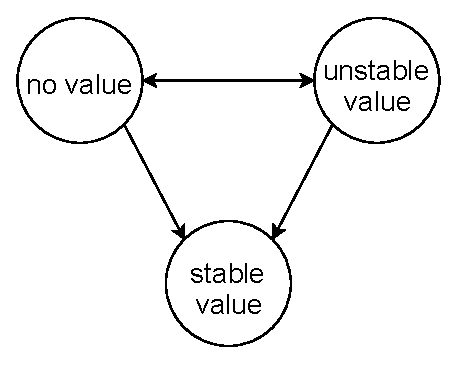
\includegraphics[scale=0.7]{thesis/img/task_value.eps}
\end{center}
\caption{Possible states of a \texttt{TaskValue}}
\label{fig:task_value}
\end{figure}

A Task can be of any type, as long as there is an instance of the \texttt{iTask} type class to it. This instance can be automatically derived or explicitly declared. Automatic derivation is available for any type as long as it is not abstract, extendable or the function type. Basic types have instances already declared in the iTasks library. Explicit declaration allows the user to define a custom instance of the \texttt{iTask} type class if the default derived instance is not suitable. In addition, it allows instances for extendable, abstract and the function types. 

\section{Interaction}\label{interaction}

The iTasks library provides basic tasks for interacting with the user. Listing \ref{l_top1} shows the three basic interactive tasks: \texttt{enterInformation}, \texttt{viewInformation} and \texttt{updateInformation}. They create user interface elements to enter, view and update information respectively. Notice that on all of the taks below, there is a constraint which requires that the type \texttt{m} of the returned \texttt{Task} must implement an instance of the \texttt{iTask} type class. 

\begin{lstlisting}[caption=iTasks basic interaction functions,captionpos=b,label=l_top1]
class toPrompt d where
    toPrompt :: !d -> UI

enterInformation :: !d ![EnterOption m] -> Task m | toPrompt d & iTask m
viewInformation :: !d ![ViewOption m] !m -> Task m | toPrompt d & iTask m
updateInformation :: !d ![UpdateOption m m] m -> Task m | toPrompt d & iTask m 
\end{lstlisting}


Listing \ref{l_top2} displays examples of how to use these tasks. We introduce a new \ac{adt}, called \texttt{Location} and automatically derive its instance of the \texttt{iTask} type class. Following, we introduce a new example location. Finally, we define tasks based on the basic tasks defined in Listing \ref{l_top1}. Here, keep in mind that the iTasks standard library implements an instance of the \texttt{toPromt} type class for the type \texttt{String}.  


\begin{lstlisting}[caption=Example of basic iTask interaction functions,captionpos=b,label=l_top2]
:: Location = { city :: String, state :: String }

derive class iTask Location

location :: Location
location = { city="Omaha", state="Nebraska"}

enterLocation :: Task Location
enterLocation = enterInformation "Enter the location" []

viewLocation :: Task Location
viewLocation = viewInformation "View the location" [] location

updateLocation :: Task Location
updateLocation = updateInformation "Update the location" [] location
\end{lstlisting}

Figure \ref{fig:itasks_display} displays the user interfaces generated for the basic tasks \texttt{enterInformation} (Figure \ref{fig:enter_info}), \texttt{viewInformation} (Figure \ref{fig:view_info}) and \texttt{updateInformation} (Figure \ref{fig:upd_info}).

\begin{figure}[H]
\begin{subfigure}{0.33\textwidth}
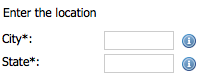
\includegraphics[scale=0.7]{thesis/img/enter_location.png}
\caption{Enter Information}
\label{fig:enter_info}
\end{subfigure}
\begin{subfigure}{0.33\textwidth}

\includegraphics[scale=0.55]{thesis/img/view_location.png}
\caption{View Information}
\label{fig:view_info}
\end{subfigure}
\begin{subfigure}{0.33\textwidth}
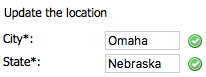
\includegraphics[scale=0.7]{thesis/img/update_location.png}
\caption{Update Information}
\label{fig:upd_info}
\end{subfigure}
\caption{The visual representation of the basic iTask interaction functions}
\label{fig:itasks_display}
\end{figure}


\section{Combinators}\label{combinators}

Although the basic tasks introduced in Section \ref{interaction} allow the user to exchange information with the iTasks application, they are quite limited. In order to allow the user to express more complex behavior, task combinators were introduced. Combinators are functions (usually infix operators) that determine how its argument tasks will be combined into a new task. There are only two fundamental combinators, sequence and parallel. All the other combinators in the \texttt{iTask} library are defined based on these fundamental combinators.

\subsection{Sequential Combinator}
\begin{lstlisting}[caption=Sequential Combinators,label=seq_comb,captionpos=b]
(>>*) infixl 1 :: !(Task a) ![TaskCont a (Task b)] -> Task b | iTask a & iTask b

:: TaskCont a b                               
	= OnValue ((TaskValue a) -> Maybe b)         
	| OnAction Action ((TaskValue a) -> Maybe b) 
	| E.e: OnException (e -> b) & iTask e        
	| OnAllExceptions (String -> b)    
\end{lstlisting}

\subsection{Parallel Combinators}

\begin{lstlisting}[caption=Parallel Combinators,label=par_comb,captionpos=b]
(-||-) infixr 3 :: !(Task a) !(Task a) -> Task a | iTask a
(-&&-) infixr 4 :: !(Task a) !(Task b) -> Task (a,b) | iTask a & iTask b
\end{lstlisting}


\section{Shared Data Sources}


\chapter{The mTask EDSL}
    In some cases, interactions between the iTasks system and the real world could be automated. This is the case for tasks such as reading the room temperature or turning a \acs{led} on once a task is completed. Microcontrollers are perfect for this kind of task. They are cheap systems that great for control tasks that involve reading sensors (e.g., temperature, light) and controlling actuators (e.g., motors, \acsp{led}). Due to hardware limitations, microcontrollers can not run iTasks tasks. As an alternative, the mTask \ac{edsl} was created. This \ac{dsl} allows the programming of microcontrollers in Clean using a TOP-like approach~\cite{micro,mtasks,martthesis}.

The mTask \ac{dsl} is a type safe, class-based, multi-view \ac{edsl} (Section \ref{sec:class_based_edsl}). It currently has three views: C++ code generation, evaluation and interpretable bytecode generation. An overview of the views is given in Section \ref{sec:mtask_views}.

\section{The Language}
Because mTask is a shallowly \ac{edsl}, language constructs are represented as functions in the host language. Instead of using functions directly, mTask is composed by type constructor classes, as described in Section \ref{sec:class_based_edsl}. A mTask type constructor class can be seen on Listing \ref{mtask_class}. In this example, the \texttt{arith} class is partially presented. An overview of mTask classes will be presented in Section \ref{sec:mtask_classes}.

\begin{lstlisting}[caption=A mTask class,captionpos=b,label=mtask_class]
class arith v where
    lit :: t -> v t Expr                             | mTaskType t                       
    (+.) infixl 6 :: (v t p) (v t q) -> v t Expr     | type, +, t & isExpr p & isExpr q
\end{lstlisting}

Language constructs are of the form \texttt{v t p} where \texttt{v} is the view, \texttt{t} is the type of the construct and \texttt{p} is the construct's role. The \texttt{lit} function lifts a value to the mTask domain. The \texttt{+.} infix operator adds two expressions (represented by the \texttt{isExpr} class constraint) and returns another expression. The constraints \texttt{type} and \texttt{mTaskType} ensure that only mTask types can be used. The constructor role specifies whether the constructor is an updatable, an expression or a statement~\cite{mtasks,martthesis}. The definitions of the constructor roles and the \texttt{isExpr} class along with its instances can be seen in Listing \ref{mtask_roles}.

\begin{lstlisting}[caption=mTask construction roles, captionpos=b,label=mtask_roles]
:: Upd   = Upd
:: Expr  = Expr
:: Stmt  = Stmt

class isExpr a :: a
instance isExpr Upd
instance isExpr Expr
\end{lstlisting}

Views are instances of mTask classes. Due to the multi-class nature of mTask, a view can choose which language constructs it supports by selecting which classes it implements. Moreover, new language constructs can be added to the language without the need to change existing code. 


\subsection{Overview of the Classes}\label{sec:mtask_classes}

The mTask \ac{edsl} is formed by many type constructor classes. Here, only the classes that are most relevant to the research are presented. Some class constraints were omitted to ease understanding.

\paragraph{Expression:} There are two classes to create expressions in mTask: \texttt{arith} and \texttt{boolExpr}. They model constructs for arithmetic and boolean expressions respectively. The \texttt{arith} class contains operators for addition, multiplication, subtraction and division in addition to a function to lift values to the mTask domain. The \texttt{boolExpr} contains operators over booleans (e.g., conjunction and disjunction) in addition to equality and inequality operators. Shortened versions of these classes can be seen in Listing \ref{mtask_expr}. 

\begin{lstlisting}[caption=mTask expression classes,captionpos=b,label=mtask_expr]
class arith v where
	lit :: t -> v t Expr 
	(+.) infixl 6 :: (v t p) (v t q) -> v t Expr | + t
	...

class boolExpr v where
	(&.) infixr 3 :: (v Bool p) (v Bool q) -> v Bool Expr 
	Not           :: (v Bool p)            -> v Bool Expr 
	(==.) infix 4 :: (v a p) (v a q)       -> v Bool Expr | == a
	(<.)  infix 4 :: (v a p) (v a q)       -> v Bool Expr | < a
	...
\end{lstlisting}

\paragraph{Control flow:} The \texttt{IF} class implements \textit{if} constructs. The \texttt{IF} function implements a \textit{if-then-else} statement and the \texttt{?} infix operator implements an \textit{if-then} statement. Given that mTask tasks can be executed periodically, loop constructs are unnecessary and are not part of mTask. The \texttt{seq} class contains the the monadic bind operator (\texttt{>>=.}) for mTask. In addition, it contains a variant of the monadic operator where the result of its first argument is disregarded. This operator is equivalent to the semicolon in imperative languages. The \texttt{retrn} class contains a single function that terminates the task. Control flow classes can be seen in Listing \ref{mtask_contr}

\begin{lstlisting}[caption=mTask control flow classes,captionpos=b,label=mtask_contr]
class IF v where
  IF :: (v Bool p) (v t q) (v s r)  -> v () Stmt | isExpr p
  (?) infix 1 :: (v Bool p) (v t q) -> v () Stmt | isExpr p
class seq v where
  (>>=.) infixr 0 :: (v t p) ((v t Expr) -> (v u q)) -> (v u Stmt) 
  (:.) infixr 0 :: (v t p) (v u q) -> v u Stmt 
class retrn v where
  retrn :: v () Expr
\end{lstlisting}

\paragraph{\aclp{sds}} The \texttt{sds} class contains functions to create \aclp{sds}. The \texttt{sds} function is used to create updatable \acp{sds} and the \texttt{con} function is used to create constant \acp{sds}. Both use the technique described in Section \ref{sec:class_based_edsl} to guarantee a type-safe usage of \acp{sds}. The \texttt{sdspub} class contains a construct to publish \acp{sds}. The \texttt{assign} class contains a single function to enable assignment in mTask. \ac{sds} classes can be seen in Listing \ref{mtask_sds}. Notice that the functions below enforce the construct role \texttt{Upd} to ensure that only updatables are used.

\begin{lstlisting}[caption=mTask SDS classes,captionpos=b,label=mtask_sds]
:: In a b = In infix 0 a b
:: Main a = {main :: a}

class sds v where
  sds :: ((v t Upd)  -> In t (Main (v c s))) -> (Main (v c s))
  con :: ((v t Expr) -> In t (Main (v c s))) -> (Main (v c s)) 
class sdspub v where
  pub :: (v t Upd) -> v t Expr
class assign v where
  (=.) infixr 2 :: (v t Upd) (v t p) -> v t Expr | isExpr p
\end{lstlisting}

\paragraph{Input and output} There are constructs to handle both analog and digital input and output. The classes \texttt{dIO} and \texttt{aIO} contain functions to handle digital and analog I/O, respectively. Both classes create updatables that can be used to read from and write to a pin. The \texttt{userLed} class contains functions to turn \acsp{led} on an off. Input/output classes can be seen in Listing \ref{mtask_io}. 

\begin{lstlisting}[caption=mTask I/O classes,captionpos=b,label=mtask_io]
:: DigitalPin = D0 | D1 | D2 | D3 | D4 | D5 |D6 | D7 | D8 | D9 | D10 | D11 | D12 | D13
:: AnalogPin  = A0 | A1 | A2 | A3 | A4 | A5
:: UserLED   = LED1 | LED2 | LED3

class dIO v where
	dIO :: DigitalPin -> v Bool Upd
class aIO v where
	aIO :: AnalogPin  -> v Int Upd
class userLed v where
  ledOn  :: (v UserLED q) -> (v () Stmt)
  ledOff :: (v UserLED q) -> (v () Stmt)
\end{lstlisting}


\subsection{Overview of the Views}\label{sec:mtask_views}

Currently, mTask has three views: C++ code generation, evaluation and bytecode generation.

The C++ code generation view translates language constructs to Arduino's dialect of C++. The Arduino IDE compiles the C++ source code to machine code for the microcontrollers. 
It is convenient to generate C++ code instead of machine code because it saves us from the task of generating code for different microcontrollers. In addition, C++ gives us the level of control we need to handle low level input/output operations. This view consists of a function that modifies a compilation state, \texttt{CODE}. The state is a record that stores the generated code along with some information to generate identifiers and to keep track of source code indentation. At the end of compilation, the \texttt{CODE} record is transformed into C++ code which can be saved into disk, loaded into the Arduino IDE and uploaded to microcontrollers.


The evaluation view translates language constructs into Clean programs. It consists of a function that modifies an evaluation state. The state is a record that stores tasks, program variables and input/output information. Given that programs running on microcontrollers are hard to debug, one can benefit from this view to find program errors. This view can be used to build a mTask simulator using iTasks where the user can observe the state of the program on each loop of the microcontroller.

The last mTask view transforms language constructs into interpretable bytecode. Since the research focused on this view of mTask, it will be discussed in more detail in Section \ref{sec:int_mtask}.

\section{Interpreted mTask}\label{sec:int_mtask}

\subsection{Motivation}

Although the C++ code generation view works as expected, it poses a limitation. Tasks generated by this view are static: once they are compiled and uploaded, they cannot be changed. If the user wishes to change the current task or add new tasks to the microcontroller, the program has to be recompiled and reuploaded. This presents two problems. First, microcontrollers have a limited amount of write cycles in their program memory~\cite{martthesis}. Therefore, repeated uploading of new programs is not desired. Second, due to the nature of microcontrollers and the \ac{iot}, such devices are often located on places that are hard to reach. Therefore, it is not desirable that every time a new task has to be uploaded, the device has to be physically reached, plugged into a computer and put back in place.

To overcome that limitation, a new view of mTask was created~\cite{martthesis}. This view generates interpretable bytecode rather than C++ code. The bytecode can be interpreted by a runtime system in the device (the \textit{client}). This runtime system (the \textit{engine}), is written in C and can be compiled and uploaded using the Arduino IDE. Tasks and \acp{sds} are sent to the client dynamically. Therefore, devices are programmed once but can execute tasks dynamically. Additionally, this setting can be more robust than the static mTask. If the communication with a device fails, the server can dynamically send the tasks that were running on it to another suitable device. 

\subsection{Communication Protocol}

Devices can be connected either via serial communication or TCP. The server and the client communicate via a protocol based on messages. Incoming messages are of type \texttt{MTaskMSGSend} --- messages are always named from the server's perspective. There are messages for task addition and deletion, shutdown request, \ac{sds} addition and update and specification request. The definition of the \texttt{MTaskMSGSend} \ac{adt} can be seen in Listing \ref{msg_send}.

\begin{lstlisting}[caption=Communication protocol: sent messages,captionpos=b,label=msg_send]
:: BCValue = E.e: BCValue e & mTaskType e

:: MTaskMSGSend = 
      MTTask MTaskInterval String
    | MTTaskDel Int
    | MTShutdown
    | MTSds Int BCValue
    | MTUpd Int BCValue
    | MTSpec
\end{lstlisting}

The client communicates with the server via messages of type \texttt{MTaskMSGRecv}. There are messages for task acknowledgment and deletion, \ac{sds} acknowledgment, deletion and publication, debugging messages, device specification and empty messages. The definition of the \texttt{MTaskMSGRecv} \ac{adt} can be seen in Listing \ref{msg_rec}. The \texttt{MTaskDeviceSpec} data type contains the specification of the device, i.e. its stack size, memory size, number of digital and analog pins.

\begin{lstlisting}[caption=Communication protocol: received messages,captionpos=b,label=msg_rec]
:: MTaskMSGRecv = 
      MTTaskAck Int Int
    | MTTaskDelAck Int
    | MTSDSAck Int
    | MTSDSDelAck Int
    | MTPub Int BCValue
    | MTMessage String
    | MTDevSpec MTaskDeviceSpec
    | MTEmpty
\end{lstlisting}

\subsection{The Client}

The client runs a loop function that runs repeatedly until a \textit{shutdown} message is received. The loop consists of two pieces: checking for incoming messages and running the task scheduler. The first step is straightforward: it checks the input buffer and processes any messages that might be in it. The task scheduler runs tasks based on task intervals. Tasks can run once (\texttt{OneShot}), repeatedly based on an interval (\texttt{OnInterval}) or based on an interruption (\texttt{OnInterrupt}). The interpreter is responsible for the execution of a task's bytecode.

\subsection{The Simulator}

During my Research Internship, I developed an iTask simulator for the interpreted mTask. The motivation behind it is the same as the simulator for the static mTask: programs running in microprocessors are hard to debug. The simulator mimics the C engine in many aspects, including communication, task scheduling and instruction interpretation. 

The simulator provides a web interface where the user can inspect the communication channels and the simulator state. The simulator state contains data about the simulator clock, memory, stack, tasks, \acp{sds} and peripherals (pins, LED, etc). The web interface allows peripheral values to be set manually. This is a great addition to the mTask development environment, given that sensor values can not be easily simulated on microcontrollers. In addition, users can set breakpoints on bytecode instructions and inspect the state of the simulator on specific points.

The simulator offers two modes: manual and automatic. Manual mode requires user interaction via the web interface to run. Manual simulation can be performed via either big or small steps. These two step options offer different levels of abstraction to the user. Big steps execute one entire engine loop at a time. Small steps execute each bytecode instruction individually. Automatic mode executes the simulator without the need of user interaction. It is particularly useful when the programmer needs to simulate a device but does not want to step manually through its execution. Many simulators on different modes can run simultaneously.

\section{Examples}

Two examples of mTask tasks can be seen in Listing \ref{mtask_examples}. The first example, \texttt{switch}, turns an LED on and off based on a switch connected to to digital pin \texttt{D0}. The second example, \texttt{curtains}, opens and closes curtains based on the room lighting. The curtains' controller is connected to digital pin \texttt{D0} and the light sensor is connected to analog pin \texttt{A0}. When the light sensor value is greater then 3, the curtains open. Otherwise, the curtains close. In addition, an alarm (represented by the \texttt{alarm} \ac{sds}) is triggered when the curtains open. Once the curtains open and the alarm is triggered, the task terminates.

\begin{lstlisting}[caption=Examples of mTask tasks,captionpos=b,label=mtask_examples]
switch :: Main (v () Stmt) 
switch = { main = 
	IF (dIO D0) (
		ledOn (lit LED1)
	) (
		ledOff (lit LED1)
	)}
	
curtains :: Main (v () Stmt)
curtains = sds \alarm=False In { main = 
	IF (aIO A0 >. lit 3) (
		dIO D0 =. (lit True) :.
		alarm =. lit True :.
		pub alarm :.
		retrn
	) (
		dIO D0 =. (lit False)
	)}
\end{lstlisting}



\chapter{The Application}
    The first step to answer the research question was to choose an application to develop. This chapter presents the criteria used in the selection process and the application chosen: home automation.

\section{Selection Criteria}\label{sec:selec_cri}

The application developed during the research should ideally display characteristics inherent to \acs{iot} applications~\cite{survey,survey2,survey3}. Although, some of there characteristics --- energy consumption, performance and security --- were not considered during the research. These aspects were ignored because the development of \gls{iTasks} overlooked them. Additionally, some criteria were added based on the research question.

The following criteria were used to choose an application:

\paragraph{Suitable} The application should solve a problem that is suitable for \gls{mTask}. This narrows the choice to \ac{iot} applications that can be developed for platforms supported by \gls{mTask}.

\paragraph{Non-trivial} Trivial applications (e.g. an \acs{led} blinking) were previously developed~\cite{martthesis}. Therefore, the application should not solve a trivial problem --- e.g. a simple hallway  motion-activated light sensor. It should go beyond a purely reactive system. It does not have to solve a novel problem, but its development should be adequately challenging.

\paragraph{Simple} Due to time constraints, it should be simple enough to be developed during this research. Since building a full-pledged application is not the goal of the research, some concerns as feature completeness, user experience design and security are not taken into account. Its source code should not be too complex.

\paragraph{Interesting} It is not enough that the application is suitable and technically good. It should tackle an existing, interesting problem. Ideally, a problem which users inserted into the application domain would be willing to pay for a solution.

\paragraph{Significant} The application should somehow improve the environment it is inserted into. Examples are accelerating an assembly line, saving commute  time, improving one's health or well being or reducing operational cost.

\paragraph{Comprehensible} Its domain and main features should be easily understandable by non-domain experts. Its functionality details and operational features might require specific knowledge, but the application should be easily described on a high level to someone who is not inserted in its domain. Comprehensibility is relevant because it improves the application and therefore the research's reachability. 

\paragraph{Robust} The application should be able to handle errors to some extent. It should at least be able to detect and communicate device disconnection. Ideally, it would automatically migrate tasks from disconnected devices to available devices whenever possible. 

\paragraph{Highly connected} It should support multiple devices simultaneously. These devices should be able to exchange information (e.g. sensor values) when suitable. Ideally, the devices would be connected wirelessly.

\paragraph{Dynamic} The application should not be static. Given that the interpreted version of \gls{mTask} (Section \ref{sec:int_mtask}) is being explored, its dynamic nature should be exploited. The application domain should naturally allow dynamicity. Ideally, tasks would be sent to and removed from devices regularly.

\paragraph{Diverse} It should use as many peripherals as possible. Since \gls{mTask} targets microcontrollers, it is important that a diverse group of sensors and actuators is used. The application should not restrict itself to a couple of peripherals. 

\paragraph{Extensive} The application should use \gls{mTask} features extensively. Given that it is testing \gls{mTask}'s capabilities, it is important that the application tests as many \gls{mTask} features as possible. There is a correlation between the number of features used by the application and the certainty about \gls{mTask}'s abilities.

\section{Home Automation}

Many potential \ac{iot} applications were considered to be developed during research. After a systematic selection process based on the selection criteria described on Section \ref{sec:selec_cri}, a home automation solution was chosen. A detailed analysis of why this domain was chosen is presented in Section \ref{sec:app_analysis}.

Home automation might refer to different levels of automation of home tasks. By definition, any tool or machine that automates a home task constitutes a home automation solution. Historically, home automation became popular with the advent of distributed electricity. Daily tasks as dishwashing and drying clothes were automated by appliances that today are common in many households around the world.

In the last decades, home automation gained another meaning with the invention of electronic solutions that control virtually any electronic in a house. Lighting, air conditioners, heaters, entertainment systems and doors are common components controlled by home automation solutions. Frequently, these systems are composed by a central control unit with a user interface (e.g. computer, tablet, smartphone, wall control panel), a communication channel (e.g. Bluetooth, \acs{lan}, Internet, infrared) and devices to be controlled (e.g. lamp, air conditioning unit, doors, TV, appliances).

Automated tasks might be as simple as turning a light on when someone enters the room, controlling the heater based on a target room temperature, locking the main door at a set time and closing the curtains based on the amount of natural light outside. They might also be more elaborated as automatically turning the coffee maker on at 8:00 AM on work days, but only if somebody is at home.

\section{Application Description}\label{sec:app_desc}

The home automation application developed is called Autohouse. It enables and manages the automation of a home (hereafter referred to as \textit{smarthome}) using \gls{mTask}. A smarthome is composed by rooms that can be added and removed by its user. Each room contain devices (called \textit{units} in the application) that execute tasks chosen by the user. 

A smarthome is managed via the control panel, a web interface that can be accessed using a web browser. Multiple instances of the control panel can run simultaneously. There, the user has access to the main features of the application:

\begin{itemize}
    \item Manage home: add and remove rooms to the smarthome.
    \item Manage room: add and remove units to a room.
    \item Send task: send a new task to one of the available units.
    \item Inspect unit: see which tasks are running on a unit.
\end{itemize}

\subsection{Architecture}

Autohouse is a centralized solution: a server (ideally located in the home) is the central communication hub for both users and devices. User communication is accomplished via the web control panel, which is hosted in the server. Device communication is accomplished via the \gls{mTask} library and its communication protocol described in Section \ref{sec:mtask_com_prot}. Figure \ref{fig:autohouse_arch} displays an example architecture of Autohouse deployed on a home with three units. 

\begin{figure}[H]
\begin{center}
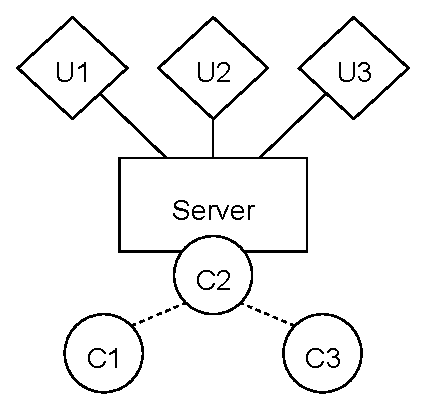
\includegraphics[scale=1.0]{thesis/img/autohouse_arch.eps}
\end{center}
\caption{Autohouse Architecture}
\label{fig:autohouse_arch}
\end{figure}

In Figure \ref{fig:autohouse_arch}, units are represented as diamonds, the server is represented as a rectangle and clients accessing the web control panel are represented as circles. Rooms are just an abstraction layer to ease the use of Autohouse and therefore are not represented in its architecture. Units are microcontrollers equipped with peripherals (sensors, actuators) and with a communication interface. The server can be any computer with networking capabilities that is supported by \gls{clean} and that has enough resources to run the application. A client is a device accessing the control panel using a web browser. Note that the server itself may be a client, since it can access the control panel via a web browser. In addition, if the server is exposed to the Internet, the control panel can be accessed remotely. 

Communication between the server and the units must be persistent (represented by the continuous line between them in Figure \ref{fig:autohouse_arch}). If the communication is interrupted, the server interprets it as a disconnection. Communication between the server and the clients can be transient (represented by the dotted line between them in Figure \ref{fig:autohouse_arch}). Since clients are just managing the application, their connection does not have to be persistent. 

Following one of the criterion introduced in Section \ref{sec:selec_cri}, units should connect to the servers wirelessly. The \gls{mTask} library supports two types of connections: Serial and \acs{tcp}. Although, which technology is used to establish these connections is irrelevant to the end user. Therefore, Autohouse is technology agnostic in regard to communication between units and the server. Units can, for example, establish a serial connection via Bluetooth or a \acs{tcp} connection via WiFi. As a consequence, Autohouse does not enforce a wireless connection between the units and the server. The user decides which communication technology is more adequate to their needs.

\subsection{Tasks}

The main purpose of Autohouse is to send automation tasks to units so they can be executed without human supervision. Therefore, the tasks the application supports play a key role in Autohouse. The application has a list of predefined tasks that are relevant to the house automation domain. The user can pick tasks from this default task list and select a unit to send it to. The standard task list might be extended by adding new tasks to the \texttt{Programs} module. The \gls{autohouse} standard tasks are listed below.

\begin{itemize}
    \item Control a light based on a switch. 
    \item Turn a light on when movement is detected.
    \item Lock a door when it gets dark.
    \item Open the garage door if a car is reversing.
    \item Turn a fan on when it gets humid enough, but turn it off when something is about to hit it.
    \item Open and close windows based on a target temperature range.
    \item Open and close curtains based on the amount of light in the room.
    \item Manage the air conditioning unit and the heater based on a target room temperature and on the actual room temperature.
\end{itemize}

\subsection{Devices}\label{sec:autohouse_devices}

Three platforms are supported by mTaks: \gls{arduino}, \acs{posix} and \gls{mbed}. \gls{arduino}~\cite{arduino} was chosen as the main platform for Autohouse. \gls{arduino} is an open-source electronics prototyping platform which has single-board microcontrollers specifications and software to support them. It was chosen because of its open-source nature, popularity, well-established community and open-source code availability.

The \gls{arduino} platform currently has many boards with different specifications and purposes. The \gls{arduino} Uno Rev3\footnote{Arduino Uno Rev3. Available at \url{https://store.arduino.cc/arduino-uno-rev3}. Accessed on August 26th 2018.} was chosen as the target device because of its popularity, extensibility (using shields\footnote{Arduino Shields. Available at \url{https://www.arduino.cc/en/Main/arduinoShields}. Accessed on August 26th 2018.}), cost and limited resources. The \gls{arduino} Uno is based on the ATmega328P microprocessor, which has only 2 KB of RAM. This memory limitation is a desired characteristic, given that \gls{mTask}'s suitability for microcontrollers is being tested and that such devices might have extremely limited resources. The \gls{arduino} Uno operates at a frequency of 16 MHz, has 6 analog pins, 14 digital pins, 32 KB of flash memory and a built-in \acs{led}. Its digital and analog pins are often used to interface with peripherals, including sensors and actuators. 



Sensors and actuators are extremely relevant to Autohouse because they allow the application to interface with the real world without human interference. Examples of sensors are temperature, humidity and movement sensors. Examples of actuators are buttons, switches, \acsp{led} and motors.

\subsection{Sensors}

\gls{autohouse} relies on the interpreted \gls{mTask} and its \gls{arduino} client for peripheral support. Therefore, it supports the same sensors the \gls{arduino} client does. Digital and analog pins can be controlled explicitly, but \gls{mTask} also provides native support for some sensors. Namely, for the DHT22 temperature and humidity sensor, the HCSR04 ultrasonic sensor, digital light sensor, Grove analog light sensor (P) V1.1 and \ac{pir}. Native sensor support allows programming in a high level of abstraction, in which sensor values represent their semantics. For example, reading from a temperature sensor returns a \texttt{Temperature}, an \acs{adt} that represents temperature in Celcius. Some of these sensors were not previously supported by \gls{mTask}. Section \ref{sec:new_peri} describes how these peripherals were incorporated into \gls{mTask}.

\subsection{Actuators}

Similarly to sensors, \gls{autohouse} relies on the interpreted \gls{mTask} and its \gls{arduino} client for actuator support. Some actuators (e.g. switches, buttons) can be directly controlled through pins and therefore do not require custom support. Other actuators, though, require custom support to be practically used. The interpreted \gls{mTask} provides native support for \acs{lcd} displays (to print integers only), \acsp{led} and servos. Servos were not previously supported by \gls{mTask}. Section \ref{sec:new_peri} describes how servos were incorporated into \gls{mTask}.

\section{Application Analysis}\label{sec:app_analysis}

The selection process that chose Autohouse as the research application was guided by the selection criteria presented in Section \ref{sec:selec_cri}. In this section, the Autohouse choice is motivated by analyzing the application under those same criteria.

\paragraph{Suitable} Autohouse is suitable for \gls{mTask}. Its components are small devices connected to a server that (if connected to the internet) can be accessed anywhere. In addition, Autohouse targets \gls{arduino} Uno, a board supported by \gls{mTask}.

\paragraph{Non-trivial} It is not a trivial application. The complexity of Autohouse goes beyond a simple reactive system. It is an application with a user interface where its user can dynamically add devices and send automation tasks to such devices. Its tasks can be simple reactive tasks but can also contain complex logic based on input from different sensors and devices.

\paragraph{Simple} Autohouse was simple enough to be developed during the research. Thanks to the prototyping nature of \gls{iTasks}, its development could abstract from many technical details and focus on design decisions.

\paragraph{Interesting} Home automation is becoming increasingly popular and its industry is growing consistently\footnote{Global Home Automation Market Growth Opportunities 2017-2022 - Market is expected to reach an estimated \$75.2 billion. Available at \url{https://markets.businessinsider.com/news/stocks/global-home-automation-market-growth-opportunities-2017-2022-market-is-expected-to-reach-an-estimated-75-2-billion-1007431226}. Accessed on August 27th 2018.}. There is no industry standard and the market is highly fragmented. Therefore, Autohouse solves an existing, interesting problem.

\paragraph{Significant} Autohouse might improve many aspects of its user's life. For example, Autohouse tasks can save time (e.g. automatically opening the garage door when a car moves backwards). They can also save energy (e.g. automatically turn off the lights and electronics when nobody is home). They might also improve the user's well being (e.g. automatically regulate room temperature) and health (e.g. open the windows when the air quality inside is poor). In addition, tasks can be simply convenient (e.g. open the curtains when it is bright outside).

\paragraph{Comprehensible} The home automation domain is comprehensible to most people. We all live in homes and can relate to most of the tasks Autohouse offers. Therefore, no explanation of the application domain is required to comprehend it. 

\paragraph{Robust} Autohouse is a robust application when it comes to device disconnection. If a unit is disconnected from the server, the system migrates the tasks that were running on that unit to another, suitable unit. The application does not support server fault tolerance. Although the distributed version of \gls{iTasks} could have been used, Autohouse runs on the single server version instead~\cite{distributed}.

\paragraph{Highly connected} Autohouse supports multiple simultaneous devices. In the home automation domain, having many devices simultaneously connected is not only common, but encouraged. Wireless connections are supported but as explained in Section \ref{sec:app_desc}, Autohouse does not enforce them. 

\paragraph{Dynamic} The Autohouse system allows for dynamic addition and removal of devices. In addition, a user might send tasks to devices dynamically. Home automation is a domain that naturally requires dynamicity. It is expected that Autohouse users create and delete tasks on a daily basis.

\paragraph{Diverse} Autohouse supports five different sensors and three actuators. Therefore, in total, eight peripherals are integrated into the application. Although this number is small when compared to some commercial applications out there, it is enough to display Autohouse's diversity.

\paragraph{Extensive} The application tests \gls{mTask} features thoroughly. Regarding the \gls{mTask} language, \gls{autohouse}'s default tasks use all of the language constructs implemented by the \gls{mTask}'s interpreted view (Section \ref{sec:int_mtask}). In addition, it makes use of \gls{mTask} functionality to connect to devices and to send tasks to it. Autohouse benefits from \gls{mTask} abstraction layer over devices and does not handle them directly.



\chapter{Application Development}
    After the application was chosen, development began. This chapter describes the development process. Since the application was not the object under research, a quick overview of its development is given in Section \ref{sec:dev_overview}. During development, limitations of \gls{mTask} were found. Some were overcome and are described in Section \ref{sec:mtask_changes}. Other limitations remain and are described in Section \ref{sec:limitations}. Finally, Section \ref{sec:task_migration} describes how automatic task migration was accomplished without modifying \gls{mTask}.

\section{Development Overview}\label{sec:dev_overview}
\gls{autohouse} is an application developed using \gls{clean}, \gls{iTasks} and \gls{mTask}. Due to time constraints, it was thoroughly tested only on macOS 10.13 (High Sierra). It was tested on Linux (Ubuntu 16.10) on early stages of development. It was not tested on Windows at all because the CleanSerial library (which \gls{mTask} depends on) does not support it. \gls{autohouse}'s source code is available at its GitHub repository~\footnote{Autohouse on GitHub. Available at \url{https://github.com/matheusamazonas/autohouse}.}.

\subsection{Application Architecture}
\gls{autohouse} development started just like many \gls{iTasks} applications: defining \acsp{adt} and \acsp{sds}. The application has \acsp{adt} that model key concepts in the home automation domain: \texttt{House} (representing the smarthome), \texttt{Room} and \texttt{Unit} (representing a device). A \texttt{House} is a list of \texttt{Room}s and a \texttt{Room} is essentially a list of \texttt{Unit}s. 

All the application data lives in one \acs{sds} that represents the entire house. Other \acsp{sds} (e.g. for rooms and units) are derived from this main \acs{sds} using parametric lenses~\cite{parametric}. Rooms and units have unique ids that are used to locate them in the house \acs{sds}. 

The application contains three main tasks running in parallel: manage house, manage units and send new task. The first one lets the user create and edit rooms. The second allows the user to inspect, send tasks to and disconnect units. The last task lets the user pick a \gls{mTask} task to send to a device that is compatible with it.

Once the \gls{iTasks} foundation was created, the \gls{mTask} development could begin.

\subsection{Using the Simulator}
As expected, device features were first implemented using simulators (Section \ref{mtask_simulator}). These devices proved to be great for early stages of development. First, multiple simulators can be easily instantiated, which was particularly useful when physical devices were not available yet. Simulators allowed the development of peripheral tasks even before some peripherals were available for testing. Additionally, given that simulators are highly customizable, some features that depended on different device configurations were tested. Such a freedom of device setting choice does not exist when dealing with physical devices. 

Although the simulator was particularly helpful during early stages of development, it proved to be a great debug tool during later stages as well. Whenever a device behaved unexpectedly, the same environment was reproduced using a simulator. Then, using the debugging \acs{ui}, the device's state (i.e. memory, tasks, program counter, peripheral values) could be inspected. Using the simulator as a debug tool became standard practice during \gls{autohouse}'s development.

\subsection{Device Communication}
Once prototyping using the simulator was over, development moved to physical devices. But one problem had to be solved before deploying \gls{mTask} tasks on \gls{arduino}s: wireless device communication. Ideally, \gls{autohouse} would communicate with its devices wirelessly. But so far, only Serial connections over \acs{usb} were used to connect to \gls{arduino}s. Two wireless options were taken into consideration: Wi-Fi (through \acs{tcp}) and Bluetooth (through Serial).

The first option tested was Wi-Fi, specifically with the ESP8266. The ESP8266 is a system on a chip with a microcontroller, a full \acs{tcp}/\acs{ip} stack and Wi-Fi. It can be used either as a Wi-Fi module (giving other microcontrollers Wi-Fi capabilities) or as a standalone microcontroller. In \gls{autohouse}'s setting, it would be used to give the \gls{arduino} boards Wi-Fi capabilities. A microcontroller can use Hayes commands\footnote{Hayes command set - Wikipedia. Available at \url{https://en.wikipedia.org/wiki/Hayes_command_set}. Accessed on September 14th 2018.} to control the ESP8266 as a Wi-Fi module. Thus, a library was required to interface with it. A couple of open-source libraries were tested\footnote{WiFiEsp on GitHub. Available at \url{https://github.com/bportaluri/WiFiEsp/tree/master/src}. Accessed on September 14th 2018.}\textsuperscript{,}\footnote{ESP8266wifi on GitHub. Available at \url{https://github.com/ekstrand/ESP8266wifi}. Accessed on September 14th 2018.}, but they either did not offer some necessary features (e.g. retrieve the list of connected clients) or behaved unexpectedly (e.g. losing received messages). After some unsuccessful attempts to adapt the existing libraries, Wi-Fi was put aside and Bluetooth was considered as an alternative.

The Bluetooth module tested was the HC-05, a Bluetooth 2.0 \ac{spp} module. Since this module runs through Serial, it can be directly connected to the \gls{arduino} board's Serial pins (\texttt{TX} and \texttt{RX}). Incoming data is preprocessed by the HC-05 and send directly to the device's Serial port. Therefore, no client data processing is required to transmit data via Bluetooth. Additionally, no code changes were necessary to support Bluetooth connection. When compared to Wi-Fi, Bluetooth brought clear advantages --- i.e. it works out of the box and does not required additional code --- and therefore was chosen to be used as \gls{autohouse}'s wireless solution.

\subsection{Device Deployment}

Once the wireless communication was set up, development moved to physical devices. First, all peripherals were tested using a single \gls{arduino} board to ensure that they were compatible. Once all peripherals were tested using \gls{mTask} tasks, more devices were added to the \gls{autohouse} system. 

The test system contained five \gls{arduino} Uno compatible boards. Each board was equipped with a HC-05 Bluetooth module, two \acsp{led}, two push down buttons, a \acs{pir} and temperature, humidity, ultrasonic and analog light sensors. The boards had similar capabilities in order to test task migration (tasks should only migrate to devices that are compatible with it). Only one board was equipped with a \gls{servo}. This choice was also motivated by the task migration feature: if a device running a task that uses a \gls{servo} disconnects from the server, its task should not migrate because no other device has a \gls{servo}.

Once device deployment finished, \gls{autohouse}'s standard task list was created and tested. \gls{autohouse}'s version\footnote{\gls{autohouse} release 0.1.0 on GitHub. Available at \url{https://github.com/matheusamazonas/autohouse/releases/tag/0.1.0}.} 0.1.0 corresponds to the end of this development phase.

\section{Changes to mTask}\label{sec:mtask_changes}

Limitations of \gls{mTask} surfaced during the development of \gls{autohouse}. Some of these limitations were overcome by changing \gls{mTask}. These changes are described below.

\subsection{Variables}

Since \gls{mTask} is an imperative language, it would benefit from mutable data features. Although there are no \gls{mTask} constructs to represent variables, \acp{sds} might be used as updatable data containers. In such a setting, an \ac{sds} is created for each desired variable. This trick brings updatable data storage to \gls{mTask}, but it prompts two problems. 

First, there is no separation of concerns. Variables and \acp{sds} are by definition, different things. A variable is a \textit{local} updatable data storage in memory. An \ac{sds} is an abstraction layer over any kind of shared data, including data in memory. Using an \ac{sds} locally goes against what a \textit{shared} data source represents. Second, when \acp{sds} are sent to devices, they are not attached to a specific task. Also, on the current version of \gls{mTask}, there is no way to establish whether an \ac{sds} belongs to a given task. As a consequence, \acp{sds} are never deleted from devices. Variables, on the other hand, are always bond to a specific task and could be removed with their correspondent task altogether, saving space in the device's memory. Thus, \gls{mTask} could benefit from a language construct for variables. 

The \texttt{vari} class was created to fill this gap. It contains two functions: \texttt{vari} and \texttt{con}, representing variable and constant data storage respectively. Its definition can be seen in Listing \ref{vari_class}. From a language construct point of view, the \texttt{sds} and \texttt{vari} classes do not differ much. Both classes contain constructs that might be used as updatables and as expressions. But there are two differences between these classes. First, \texttt{vari} contains a construct for constant data: \texttt{con}. Second, \texttt{vari} functions expect a value of type \texttt{t} as its initial value (seen as the first argument of \texttt{In} in Listing \ref{vari_class}). The \texttt{sds} function expects a \texttt{(Shared t)} instead. The biggest difference between the \texttt{sds} and \texttt{vari} classes regards their behavior on the interpreted view of \gls{mTask}. Variables belong to a task and will live as long as the task lives. \acp{sds} are not bound to a task and will live in the device indefinitely. 


\begin{lstlisting}[caption=The \texttt{vari} class,captionpos=b,label=vari_class]
:: Vari  = Vari
instance isExpr Vari 
instance isUpd Vari 

class vari v where
  vari :: ((v t Vari) -> In t (Main (v c s))) -> (Main (v c s)) 
  con ::  ((v t Expr) -> In t (Main (v c s))) -> (Main (v c s))
\end{lstlisting}

Listing \ref{vari_example} displays an example of variables in \gls{mTask}: the task \texttt{blink}. This task blinks \texttt{LED1} based on the value of variable \texttt{v}. The variable \texttt{v} is created using the \texttt{vari} construct. Its value is updated using the \texttt{=.} infix operator, similarly to \acp{sds}. It can also be used as a boolean expression, as the condition to an \texttt{IF} construct.

\begin{lstlisting}[caption=Example of the usage of variables in mTask,captionpos=b,label=vari_example]
blink :: Main (v () Stmt) | program v
blink = vari \v = False In { main =
	IF (v) (
		ledOn (lit LED1)
	) (
		ledOff (lit LED1)
	) :.
	v =. Not v :. noOp
	}
\end{lstlisting}

The addition of variables to the language required changes on \gls{mTask}'s communication protocol (Section \ref{sec:mtask_com_prot}). When a task is sent to a device, its variables must be sent as well. Therefore, a \texttt{MTTask} message must include the variables used by the given task. Variables are modelled in the \texttt{BCVariable} record. A variable contains a unique (within a task) identifier and its initial value. The \texttt{BCVariable} record and the communication protocol change can be seen in Listing \ref{vari_message}.

\begin{lstlisting}[caption=Change in mTask's communication protocol to accommodate task variables,captionpos=b,label=vari_message]
:: BCVariable = { vid :: Int, vval :: BCValue }

:: MTaskMSGSend
	= MTTask Int MTaskInterval [BCVariable] String
	 ...
\end{lstlisting}

Additionally, the simulator and the client engine were modified to support task variables. When a task is received, its variables are stored. During task execution, variables are fetched and assigned similarly to \acp{sds}. When a task terminates, its variables are removed from the device.

\subsection{Peripheral Code}

The \gls{mTask} library already supported some of the peripherals \gls{autohouse} planned to use: \acsp{led}, analog and digital pins. Although, new peripherals (e.g. light, temperature and humidity sensors) were required by some of the default automation tasks. Following the natural development process of an \gls{mTask} application, these peripherals were first emulated using the simulator. As more peripherals were implemented, it was clear that the workflow required to add a new peripheral to the system could be improved.

Adding a new peripheral required changes on different parts of \gls{mTask}. An overview of the necessary changes can be seen below.

\begin{itemize}
    \item A new class that represents the peripheral is added to the language. 
    \item Depending on the peripheral, a new \ac{adt} is created to represent its values (e.g. \texttt{DigitalPin}).
    \item New bytecode instructions are created.
    \item Bytecode encodings are updated to support the new instruction and the possibly new \acs{adt}.
    \item The \texttt{MTaskDeviceSpec} record is modified to include a flag for the new peripheral.
    \item The simulator interpreter is updated to handle new bytecode instructions.
    \item The \gls{cpp} client is modified to handle the new peripheral.
\end{itemize}

The changes on the \gls{cpp} client code depended heavily on the type of peripheral being implemented. Changes on the \gls{clean} code though, were often similar. Previously, peripheral code was scattered around the \gls{mTask} library. Peripheral classes were inside the \texttt{Language} module along with possibly new \acsp{adt}. Instances of the peripheral classes for each \gls{mTask} view were in the respective view's module. The simulator interpreter contained peripheral-specific code. Bytecode encodings for basic types were mixed with encodings for peripheral data types. Overall, adding a new peripheral was particularly cumbersome and extremely error-prone. Finally, there was no separation of concerns whatsoever.

A new modular code architecture for peripherals was introduced to solve the problems described above. Each peripheral should be defined in its own module. Its type class, \acsp{adt}, bytecode encodings and view instances are defined in that same module. The simulator does not have any peripheral-specific code. Instead of explicit fields for each peripheral, the simulator state record (\texttt{SimState}) contains a list of \texttt{Peripheral}. This new data type is a wrapper around every \gls{mTask} peripheral. Its definition can be seen in Listing \ref{lis:peripheral}. 

\begin{lstlisting}[caption=The \texttt{Peripheral} class,captionpos=b,label=lis:peripheral]
:: Peripheral = E.e: Peripheral e & peripheral e

class peripheral e | iTask e where
	processInst :: BC e -> State SimState (e,Bool)
\end{lstlisting}

The \texttt{peripheral} class was created to enable the removal of peripheral-specific code from the simulator interpreter. Its only function, \texttt{processInst} defines how a peripheral should interpret bytecode instructions (\texttt{BC}). Naturally, a peripheral should only interpret instructions that are relevant to it. The simulator interpreter executes one instruction at a time. If an instruction belongs to \gls{mTask}'s core instruction set (excluding peripheral instructions), the interpreter executes it immediately. If the instruction does not belong to the core instruction set, it is assumed to be a peripheral instruction and it is presented to all simulator peripherals using the \texttt{processInst} function. Once a peripheral responds to an instruction (represented by the \texttt{Bool} on \texttt{processInst} returned value), the interpreter considers the instruction executed and stops looking for a peripheral to execute it. If no peripheral executes the instruction, an error ("instruction unknown") is thrown. 

The addition of new bytecode instructions remains outside of the peripheral module. Although technically it is possible to extend the bytecode data type (\texttt{BC}) in seperate modules, the amount of work necessary to do so outweighed the benefits it could bring. 

The development that followed the changes described above proved that the separation of concerns regarding peripheral code improved \gls{mTask}. Peripherals were added faster, with less code changes and less errors. Additionally, code maintainability increased substantially. Since peripheral code lays mostly in the same module, small changes can be performed faster and safer.

\subsection{New Peripherals}\label{sec:new_peri}

Previously, the interpreted \gls{mTask} supported the following peripherals: \acsp{led}, \acs{lcd} displays (for displaying numbers only), analog and digital pins. The standard \gls{autohouse} tasks required new peripheral support. The following peripherals were added to \gls{mTask}: DHT22 temperature and humidity sensor, HCSR04 ultrasonic sensor, digital light sensor, Grove analog light sensor (P) V1.1, \ac{pir} and \gls{servo}. 

The digital light sensor, the Grove analog light sensor and the \acs{pir} did not require an external library to be used. Their data pin is connected to board pins and their values can be read using \gls{arduino} standard functions. An additional library was required to interface with the \gls{servo}. The \gls{arduino} Servo library\footnote{Arduino Servo Library. Available at \url{https://www.arduino.cc/en/reference/servo}. Accessed on September 10th 2018.} was used. An additional library was also required to interface with the DHT22 sensor. Although there are libraries available out there, I decided to implement a small and simple one just for \gls{mTask}: DHTino\footnote{DHTino on GitHub. Available at \url{https://github.com/matheusamazonas/DHTino}. Accessed on September 10th 2018.}. This choice was motivated by the limited amount of flash memory (32 KB) on the \gls{arduino} Uno. Existing libraries support many different sensors and have many features that would not be used by \gls{mTask}. As a consequence, these libraries would take too much flash memory space. Guided by the same motivation, the Ultrino\footnote{Ultrino on GitHub. Available at \url{https://github.com/matheusamazonas/Ultrino}. Accessed on September 10th 2018.} library was created to interface with the HCSR04 ultrasonic sensor.


\subsection{Device Requirements}

Some tasks rely on certain peripherals to execute. For example, a task that regulates room temperature relies on a temperature sensor. Despite that, \gls{mTask} did not provide a mechanism to determine whether a task is compatible with a device. The \texttt{Requirements} view was created to bring this feature to \gls{mTask}. Its definition can be seen in Listing \ref{lis:requirements}. \texttt{Requirement} is a type constructor with two phantom type variables: \texttt{a} and \texttt{b}~\cite{phantom}. These type variables are required by \gls{mTask} type classes. \texttt{Requirement} is a wrapper around the device specification type \texttt{MTaskDeviceSpec}. 

Given a \gls{mTask} construct, this view will return the minimum device specification necessary to support that construct. This information can be used to determine whether a device matches the minimum specification for a task and therefore, if it is compatible with it. The \texttt{match} function (seen in Listing \ref{lis:requirements}) does exactly that. Given an \gls{mTask} program and a \texttt{Maybe MTaskDeviceSpec}, it yields whether the device and program are compatible.

\begin{lstlisting}[caption=The \texttt{Requirements} view,captionpos=b,label=lis:requirements]
:: Requirements a b = Req MTaskDeviceSpec

match :: (Main (Requirements a b)) (Maybe MTaskDeviceSpec) -> Bool

instance arith Requirements
instance UserLED Requirements 
\end{lstlisting}

Instances of \gls{mTask} classes (including peripheral classes) are defined for \texttt{Requirement}. Therefore, given a \gls{mTask} task, an application can filter the available devices based on whether they are compatible with it. The opposite is also possible: given a device, an application can filter tasks based on whether they are compatible with it.

\subsection{Device Disconnection}

By design, \gls{autohouse} should be robust regarding device disconnection (Section \ref{sec:app_analysis}). Ideally, the system would detect a device disconnection and migrate the device's tasks to another suitable device. There were two challenges to tackle in order to implement this feature. 

First, \gls{mTask} does not recognize device disconnection for all of the device types it supports. Simulators never get disconnected. \acs{tcp} devices throw an \gls{iTasks} error when a disconnection is identified. This error is not caught by mTask and propagates upwards. Serial devices kill the application when disconnected. The library used by \gls{mTask} to connect to Serial devices (CleanSerial\footnote{CleanSerial on GitLab. Available at \url{git@gitlab.science.ru.nl:mlubbers/CleanSerial.git}. Accessed on Semtember 8th 2018}) halts execution when a device is disconnected. 

In order to detect device disconnection, \gls{mTask} had to be modified. If the device communication fails, the \texttt{channelSync} task (Section \ref{sec:mtask_devices}) should throw an exception\footnote{An \gls{iTasks} Task yields either a value or an exception. The \gls{iTasks} standard library provides functions to create and handle exceptions.}. \acs{tcp} devices already throw an exception when communication fails and therefore require no change. Although simulators never disconnect from the system, simulating a disconnection would benefit testing. Hence, simulators were modified to support intentional disconnection. CleanSerial was modified to support device disconnection recognition. At this point, \gls{mTask} recognizes device disconnection, but does not communicate it to \gls{autohouse}. 

Ideally, \gls{mTask} would communicate device disconnection through an error handler that would be provided by the application. Thus, the application would decide what task to perform in case of a disconnection. As seen in Section \ref{sec:mtask_devices}, the \gls{mTask} library provides a single function to connect with a device: \texttt{withDevice}. This function is responsible (besides other tasks) to manage the connection to the device and therefore was the perfect place to insert an exception handler. An exception handler is a task that takes an error \texttt{String} as input. Listing \ref{with_device} displays the type signature of the original \texttt{withDevice} along with its new version, named \texttt{withDevice'} here. 

\begin{lstlisting}[caption=Change in mTask to support a device disconnection handler,captionpos=b,label=with_device]
withDevice  :: a (MTaskDevice -> Task b)                    -> Task b | channelSync a

withDevice' :: a (MTaskDevice -> Task b) (String -> Task ()) -> Task b | channelSync a
\end{lstlisting}

Consequently, \gls{mTask} recognizes and provides an exception handler for device disconnection. \gls{autohouse} uses this feature to detect unit disconnection and thus automatically migrate tasks from the disconnected device to a suitable one.

\subsection{Simulator Improvements}\label{sec:sim_improv}

The simulator (Section \ref{mtask_simulator}) proved to be an essential tool during the development of \gls{autohouse}. Although, it was clear that it could be improved to ease debugging and testing of the application. 

Sometimes, the developer might want to debug a task and inspect it closely. The simulator's manual mode is adequate for such usage, but it might be a bit cumbersome to use. Specially with large tasks, stepping over each program instruction becomes a rather tedious and inefficient process. With that in mind, the simulator was extended to support breakpoints on bytecode instructions. Tools to add and to step over breakpoints were added to the simulator \acs{ui}. When executing a task, the simulator goes through its bytecode instructions, checking if there are breakpoints on each instruction before executing it. If an instruction has a breakpoint, execution waits for user input (by clicking on "step over") to continue. At any point, the user is able to edit breakpoints. 

The ability to simulate peripheral values is crucial for program testing in \gls{mTask}. Tasks often rely on peripheral values and therefore can only be thoroughly tested if peripheral values can be simulated. Although, the simulator did not have such feature. The development of \gls{autohouse} showed how necessary this feature is for \gls{mTask} development. Hence, simulation of peripheral values was incorporated into the simulator. Values can be manually set via the simulator \acs{ui}, similarly to breakpoints. 

\section{Limitations of mTask}\label{sec:limitations}

\section{Task Migration}\label{sec:task_migration}

In case of device disconnection, the application should migrate the unit's tasks to another suitable one. The \gls{mTask} library offers means to connect and send task to devices, but not to manage them. The application using \gls{mTask} is responsible for device management. Therefore, automatic task migration was implemented entirely in \gls{autohouse} and required no changes to \gls{mTask} whatsoever.

First, the feature behavior was defined. Although automatic task migration might me helpful, not tall tasks should be automatically migrated. For example, some tasks that are suitable for a hallway unit (e.g. motion-activated light switch) might not be suitable for a bedroom unit. Therefore, different migration strategies were created. These strategies are represented in the \texttt{Migration} \acs{adt}, seen in Listing \ref{migration_types}. 

\begin{lstlisting}[caption=Task migration strategies of \gls{autohouse},captionpos=b,label=migration_types]
:: Migration = DoNotMigrate | SameRoom | AnyRoom
\end{lstlisting}

Tasks with \texttt{DoNotMigrate} migration strategy never migrate to another unit. Tasks with the \texttt{SameRoom} strategy migrate only to units within the same room of its original unit. Tasks with \texttt{AnyRoom} strategy migrate to any other unit in the smarthome. When a task is being migrated, other units are checked for compatibility (based on the task's strategy, following no particular order) and once a compatible unit is found, the task is sent to it. The \gls{autohouse} user is responsible for determining a task's migration strategy when sending it to a unit.

The application has to save enough task data to migrate a task in case of a device disconnection. The \gls{mTask}'s \texttt{liftmTask} function (Section \ref{sec:mtask_devices}) is used to send tasks to devices. Besides the device itself, this function takes a task interval and an \gls{mTask} task as input. Therefore, this is all the information the application needs to send a task to a device. \gls{autohouse}'s default tasks have a unique id that can be used to retrieve the task from the default task list. Thus, the application only needs to store the task index and its interval (\texttt{MTaskInterval}) in order to migrate it. 

Some \gls{autohouse} tasks require user-provided arguments to work. For example, a user must provide an initial target temperature for a thermostat task before sending it to a device. If such a task is being migrated, the application should be able to restore the task arguments as well. \gls{autohouse} stores task arguments along with the task index and interval. A task's index and arguments are stored in the \texttt{ProgramData} data type. All the information necessary to migrate an \gls{autohouse} program lays in the \texttt{ProgramInstance} data type. Both data types can be seen on Listing \ref{migration_data}.

\begin{lstlisting}[caption=Task migration data,captionpos=b,label=migration_data]
:: ProgramData :== (Int, [Dynamic])   // (index, arguments)

:: ProgramInstance :== (ProgramData, MTaskInterval, Migration)
\end{lstlisting}

A unit contains a list of \texttt{ProgramInstance}s. Each list element represents one task running on the unit and can be used to migrate its respective task to a new device. If a unit disconnects, the application goes through the unit's \texttt{ProgramInstance} list and migrates the tasks accordingly. Automatic task migration was tested using simulators and physical devices and it worked as expected.

\chapter{Conclusion}
    \section{Discussion and Future Work}

\subsection{mTask}

The \gls{autohouse} application was successfully developed using \gls{mTask}, but some aspects still have to be analyzed. The tests performed during development were limited to five \gls{arduino} boards running a maximum of three simultaneous tasks for a maximum duration of one hour. It is unknown how \gls{mTask} performs running more than five simultaneous devices. Given that the number of devices in \acs{iot} applications can escalate quickly, it is important to assess how \gls{mTask} escalates in regard to the number of connected devices. Similarly, given that \acs{iot} applications often run continuously, it would be important to perform tests with tasks running for longer periods of time. Another characteristic of \acs{iot} solutions is lower power consumption~\cite{survey,survey2,survey3}. Although, no power consumption analysis of \gls{mTask} applications was performed. Assessing \gls{mTask}'s power consumption, scalability and behavior over long periods is suggested as future research. 

Ideally, the limitations of \gls{mTask} described in Section \ref{sec:limitations} should be eliminated. First, \acsp{sds} and tasks should be sent in a bundle. Thus, they would be removed altogether, eliminating dangling \acsp{sds}. Second, \gls{mTask} would avoid sending update messages to the exact same device which triggered the \acs{sds} update. Lastly, the \gls{mTask} library would provide callbacks to signal successful device connection and task acknowledgment. Solving these problems is also proposed as future research.

The Raspberry Pi\footnote{Raspberry Pi. Available at \url{https://www.raspberrypi.org}. Accessed on September 19th 2018} is a compact \acs{arm} computer often used in \acs{iot} projects both as a device and as a server. It would be interesting to see whether the Raspberry Pi is capable of running an \gls{mTask} application. Also, since the Pi hardware is Linux compatible, it might host an \gls{mTask} \acs{posix} client. Testing with the Raspberry Pi is suggested as future research.

The \gls{mTask} \acs{edsl} was created to bring \acs{iot} devices to the \gls{iTasks} environment. Its language is imperative and the system is not task-centred. Also, tasks cannot be combined as in \gls{iTasks}, limiting \gls{mTask}'s expressiveness. Naturally \gls{iTasks} and \gls{mTask} differ on some aspects, but ideally, the gap between them would be minimal, both in syntax and semantics. Current research has been performed to bridge this gap. A functional, task-centred version of \gls{mTask} has been proposed~\cite{micro}. Parallel and sequential task combinators were introduced, improving \gls{mTask}'s expressiveness. Due to time constraints, this version of \gls{mTask} could not be used in this research. Assessing the abilities of this new version of \gls{mTask} is proposed as future research.

\subsection{Autohouse}

Although \gls{autohouse} is not the research focus, it would be interesting to extend the application to push the boundaries of \gls{mTask}. 

Currently, devices have no information about what its peripherals represent. For example, a servo can be used to control curtains or to lock a door. The user might know what which peripheral represents when sending a new task to a device, but the migration algorithm does not. As a consequence, a task might migrate to a compatible device with a peripheral that controls a different object than the intended one. For example, a task that uses a servo to automatically close curtains might migrate to a device that uses its servo to lock a door. Ideally, the application user would attribute tags to its peripherals. The migration algorithm would take that information into consideration when migrating tasks.


\section{Conclusion}

The research reported in this documented tested \gls{mTask}'s ability to develop real-life \acs{iot} applications. The research question was tackled by example: the \gls{autohouse} application intended to assess \gls{mTask}'s capabilities. The application is a home automation system that allows users to dynamically manage automation tasks running on devices spread across different rooms. 

Limitations of \gls{mTask} surfaced during the development of \gls{autohouse}. Some limitations were overcome by changing the \gls{mTask} and CleanSerial libraries. Task variables were added to the language. Device disconnection recognition was implemented, allowing the application to automatically migrate tasks when a device is lost. A new view was added to the \ac{edsl} which generates minimum device requirements for a \gls{mTask} task. This view can be used to filter available devices based on whether they support a given task. Six new peripherals were added to the \gls{mTask} language and to the \gls{arduino} client. Peripheral code was restructured, easing the addition of new peripherals, increasing code maintainability and bringing a better separation of concerns between the language core constructs and peripheral constructs. Finally, the simulator for the interpreted \gls{mTask} was modified to support the setting of peripheral values and breakpoints, which improved testing and debugging considerably.

Other limitations could not be overcome during this research. \acsp{sds} are never removed from devices and live there indefinitely. There is an unwanted communication loop between devices and server whenever a device publishes an \acs{sds}. The \gls{mTask} library does not communicate neither device connection success nor task acknowledgment. Although these limitations were not overcome, they did not stop the development of \gls{autohouse}. 

The \gls{mTask} \acs{edsl} and library were successfully used to develop a real-life \acs{iot} application: the home automation system \gls{autohouse}. Some of the limitations unearthed during the development process were overcome and some remain. Finally, it is clear what the next steps to improve \gls{mTask} are.

\chapter{Related Work}
    Recent research has been conducted on mTask. A new, task-based version of it has been proposed~\cite{micro}. On this version, the imperative language has been replaced by a functional one. This new version was not used during the research reported in this document because its implementation was not available on time.

The usage of programming languages to interface with microcontrollers has been a subject of research. Firmata\footnote{Firmata Protocol Documentation. Available at \url{https://github.com/firmata/protocol}. Accessed on August 10th 2018.} is a protocol to control microcontrollers. Its messages follow the \acs{midi} message format and model mostly commands on analog and digital input and output pins. There is a client-side implementation for the Arduino\footnote{Firmara Arduino. Available at \url{https://github.com/firmata/arduino}. Accessed on August 10th 2018.} and host-side implementations for many programming languages, including a Haskell implementation to communicate with Arduinos called hArduino\footnote{hArduino. Available at \url{http://leventerkok.github.io/hArduino}. Accessed on August 10th 2018.}. Since Firmata is a protocol and not a programming language, full applications can not be built using Firmata solely. Other tools are built on top of it.

The Haskino library enables Arduino programming using Haskell~\cite{haskino}. The library is available in two different flavors. The first one is based on hArduino (and consequently, on Firmata) and requires the Arduino to maintain a serial connection with the host. On this approach, most of the program evaluation is executed on the host and only I/O commands run on the client. The second approach drops Firmata and uses its own communication protocol. The client is more independent and can execute more elaborate commands, including control flow constructs. In contrast with the first approach, it presents a lower communication overhead. In addition, programs can be written to the Arduino's \acs{eeprom}, allowing standalone execution.

Some research has been made on generating C/C++ code for microcontrollers from high level languages. Ivory is an \ac{edsl} embedded into Haskell that generates safe embedded C code~\cite{ivory1,ivory2}. By design, the generated code is memory safe and free from common errors and undefined behaviors. It uses Haskell's type system (with some \acs{ghc} extensions) to avoid errors like array indexing out of bounds, main loop function with return statements and dangling pointers. Additionally, it prohibits (by design) some standard C features that might generate unsafe code. Ivory was used on the development of the SMACCPilot, a high-assurance autopilot system for quadcopter \ac{uav}.

The \texttt{frp-arduino} library\footnote{\acs{frp} on Arduino. Available at \url{https://github.com/frp-arduino/frp-arduino}. Accessed on August 10th 2018.} implements the \ac{frp} paradigm as an \ac{edsl} embedded in Haskell. Programs in the \ac{edsl} can be compiled to Arduino C code which can be uploaded to Arduino boards. Juniper\footnote{Juniper Programming Language. Available at \url{http://www.juniper-lang.org/index.html}. Accessed on August 11th 2018.} is another \ac{frp} language for the Arduino. It is a standalone programming language that transpiles to Arduino C++.

Additionally, some programming language interpreters were ported to microcontrollers. Espruino\footnote{Espruino. Available at \url{https://www.espruino.com}. Accessed on August 10th 2018.} is a JavaScript interpreter for microcontrollers. It officially supports only proprietary boards but other microcontrollers such as the ESP8266 and the members of the STM32 family are supported by the community. Due to hardware limitations, none of the Arduino boards are supported. Espruino's official website lists many projects that were built using it, including home automation applications. 

Micropython\footnote{Micropytohn. Available at \url{https://micropython.org}. Accessed on August 10th 2018.} is a lean implementation of the Python interpreter and parts of its standard library for microcontrollers. Its main target device is the proprietary \textit{pyboard}. Given that it requires at least 16KB of RAM, it is not compatible with most Arduino boards. It is compatible with microcontrollers of the STM32 family. Many projects (including home automation) were developed using Micropython and \textit{pyboards}. 

Finally, the programming of microcontrollers dynamically (without the need to plug it to a computer) is a well known practice. For example, the ESP8266\footnote{ESP8266 Overview. Available at \url{https://www.espressif.com/en/products/hardware/esp8266ex/overview}. Accessed at August 11th 2018.} Wi-Fi module supports \ac{ota} programming. The Arduino Uno Wi-Fi\footnote{Arduino Store - Arduino Uno Wi-Fi. Available at \url{https://store.arduino.cc/arduino-uno-wifi}. Accessed on August 11th 2018.} is a version of the Arduino Uno board that contains an ESP8266 module and supports \ac{ota} programming natively via the Arduino \acs{ide}. It is important to note that although \ac{ota} enables dynamic programming of microcontrollers, it differs from mTask's dynamicity. On \ac{ota} programming, the device memory is reset when a new program is loaded. On the dynamic version of mTask, the device's memory and the tasks running on it are unaffected.

\clearpage

\nocite{*}
\addcontentsline{toc}{chapter}{Bibliography}
\printbibliography[]

%\clearpage

\printglossaries


\addcontentsline{toc}{chapter}{Listings}
\lstlistoflistings


\end{document}